\section{Гомогенное преобразование. Положение и скорость.}\label{geom}

Введем в рассмотрение объект гомогенного координатного преобразования. Здесь и далее под объектом гомогенного преобразования (англ. homogenous transform) понимается геометрическая сущность, описывающая однородное координатное преобразование, состоящее из комбинации поворота и переноса. В разных частях настоящего изложения объект гомогенного преобразования фигурирует как оператор преобразования СК, способ описания положения кинематического звена имеющий смысл соответствующего тензора, или програмный объект (в терминах ООП), непосредственно используемый в програмном обеспечении. 

Такой объект состоит из компоненты ориентации (или поворота) и компоненты трансляции (или линейного перемещения), которые в литературе обычно рассматриваются независимо. Однако, определённая общность поведения этих компонент в уравнениях движения, интуитивность обобщающего их понятия положения объекта в пространстве, а также найденные алгебраические структуры, позволяющие объединить поворот и трансляцию единой операцией композиции позволяют надеяться на возможность применения этих объектов при аналитическом решении задач в виде обособленных объектов.   

Математическое представление такого объекта может быть различным. В частности, для него могут применяться матрицы размерностью $4\times4$, бикватернионы, комбинация кватерниона поворота и вектора трансляции и т.д. В рамках рассматриваемого метода конкретная форма представления объекта взаимозаменяема и определяется исключительно удобством реализации в вычислительной системе. Обозначим объект гомогенного преобразования и соответствующий ему тензор преобразования как $H^j_i$. В програмной реализации удобно представлять $H^j_i$ как комбинацию двух компонент, кватерниона поворота и вектора трансляции.

На множестве $H^j_i$ определена операция некомутативная операция композиции, часто обозначаемая как умножение (и являющаяся умножением в терминах бикватернионов или матриц $4\times4$). Множество $H^j_i$ замкнуто по этой операции.

Введем в рассмотрение объект положения СК и связанный с ним тензор положения. Обозначим его P. Объект положения удобно задавать тем же набором компонент, что и объект гомогенного преобразования. В такой нотации компонентное выражение тензора положения $P$ j-ой системы координат взятого в i-том базисе, будет совпадать с компонентным выражением тензора преобразования СК, из базиза i-той СК в базис связанный с j-ой СК. 

\begin{equation}
P_j^{(i)} = H_{i}^{(i)j}
\end{equation}

Также введем в рассмотрение производную тензора положения j-ой системы координат

\begin{equation}\label{speed_eq} 
V_j(t) = \dot{P}_j(t) 
\end{equation}

Как и тензор преобразования системы координат и тензор положения, производная тензора положения является геометрическим объектом и имеет смысл скорости изменения геометрического положения объекта или системы координат. Часто в качестве компонентного представления производной тензора представления выбирают производные компонент тензора положения, однако такой подход не является интуитивным и не очень удобен в вычислительной реализации.

В настоящем методе в качестве компонентного представления производной тензора положения выбирается пара векторов его линейной и угловой скорости $(v,\omega)$, вне зависимости от того, какими компонентами задан сам объект положения.

\begin{equation}\label{speed_eq_comp} 
V_j(t) = |\omega_j(t),v_j(t)|
\end{equation} 

Обоснуем корректность введения такой операции дифференцирования. Рассмотрим движущийся локальный базис в базисе его мгновенного положения. Рассмотрим положение базиса через малый промежуток времени $\Delta t$. Запишем $H^j_i$ в компонентной форме через вектора поворота и трансляции.

\begin{equation}H^j_i(t) = |\rho(t), r(t)| = |0, 0|\end{equation} 
\begin{equation}H^j_i(t+\Delta t) = |\rho(t + \Delta t), r(t + \Delta t)| = |\rho, r|\end{equation} 
\begin{equation}\lim_{\Delta t \to 0}\frac{H^j_i(t+\Delta t) - H^j_i(t)}{\Delta t} = \lim_{\Delta t \to 0}|\frac{\rho}{\Delta t}, \frac{r}{\Delta t}| = |\omega, v|\end{equation} , где $\omega$ и $v$ - мгновенные угловая и линейные скорости.

Суммирование компонент вектора поворота возможно в силу колинеарности нулевого вектора любому другому вектору и тому обстоятельству, что повороты по колинеарным векторам образуют группу.

В силу тензорной природы $H^j_i$, операции над ним не зависят от выбора базиса, а значит корректна после перехода в любой выбранный базис. Воспользовавшись эквивалентностью представлений $H^j_i$, мы можем утверждать, что его производная в форме (\ref{speed_eq_comp}) существует независимо от выбора компонент представления самого $H^j_i$. Представление (\ref{speed_eq_comp}), удобно, в рамках метода, с вычислительной точки зрения, однако следует учесть, что использование такой системы компонентного представления приводит к тому, что уравнение (\ref{speed_eq}) не может быть в общем случае записано в компонентной форме, хотя бы по той причине, кто объект положения представленный кватернионом имеет 4 компоненты (а матрицей - 9), в то время как вектор угловой скорости - всего 3. Это не приводит к затруднениям, если не отходить от рассмотрения задачи в терминах самих объектов $H^j_i$, а не их компонент.

Вектор, состоящий из компонент пары векторов $(\omega, v)$ далее называется 6-вектором скорости. Альтернативное представление тензора положения в виде пары радиус вектора и вектора поворота $(r,\rho)$ далее называется 6-вектором положения.

Рассмотрим 6-вектор положения $(r,\rho)$ (порядок преобразований - сначала поворот, затем трансляция). Отметим, что, если на 6-вектор скорости $(v,\omega)$ наложить условие колинеарности 6-вектору положения $(r,\rho)$, задача может быть сведена к одномерной, дифференциальные уравнения становятся линейными, а композиции преобразований по этой 6-оси становятся комутативными и образуют группу. 
\begin{center}
  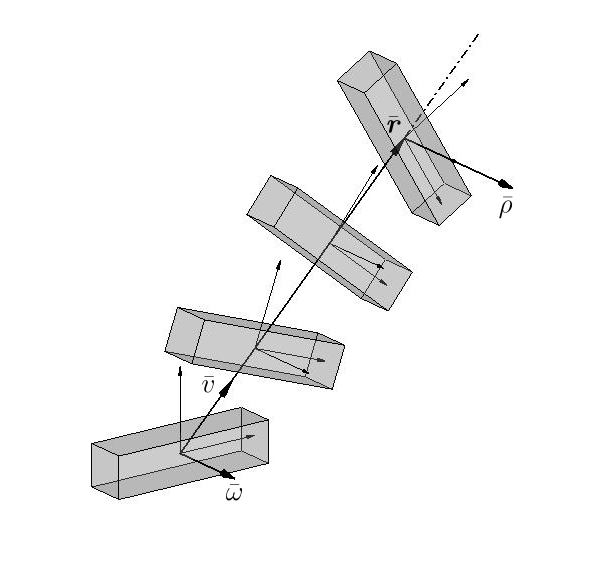
\includegraphics[width=0.8\textwidth,height=0.8\textheight,keepaspectratio]{oneaxis.png}
  \captionof{figure}{Сведение задачи к одномерному случаю.}
  \label{}
\end{center}

В форме 3-векторов для этого должны выполняться соотношения.
\begin{equation}\label{} 
\bar{v} \upuparrows \bar{r}, \  \bar{\omega} \upuparrows \bar{\rho}, \  \frac{|\bar{v}|}{|\bar{r}|} = \frac{|\bar{\omega}|}{|\bar{\rho}|} 
\end{equation}
\begin{equation}
(\bar{v_l},\bar{\omega_l}) = (\dot{\bar{r_l}},\dot{\bar{\rho_l}})
\end{equation}

Это замечание пригодится для дальнейшего изложения и может быть полезно при анализе устойчивости системы управления в терминах объектов гомогенных преобразований. 

Хочется отметить, что анализ устойчивости систем управления в терминах алгебраических объектов, отличных от действительных чисел, таких как объекты гомогенных трансформаций может иметь существенное практическое значение и представляет интересное направление исследований.